% !TEX root = ./cvl.tex
\section{Compiling CVL}

The clauses of the CVL language were introduced in Section~\ref{sec:language}. In this section we describe how the various clauses of CVL can be compiled into an \emph{execution plan} to be run on a compatible engine. There are in principle many types of plans. In this work we consider only one type of plan, namely the \emph{bottom-up} plan. 

\subsection{Bottom-up plan}

A high-level view of compiling CVL to a bottom-up plan is shown in Figure~\ref{fig:compilation}.

\begin{figure}[htbp]
\begin{center}
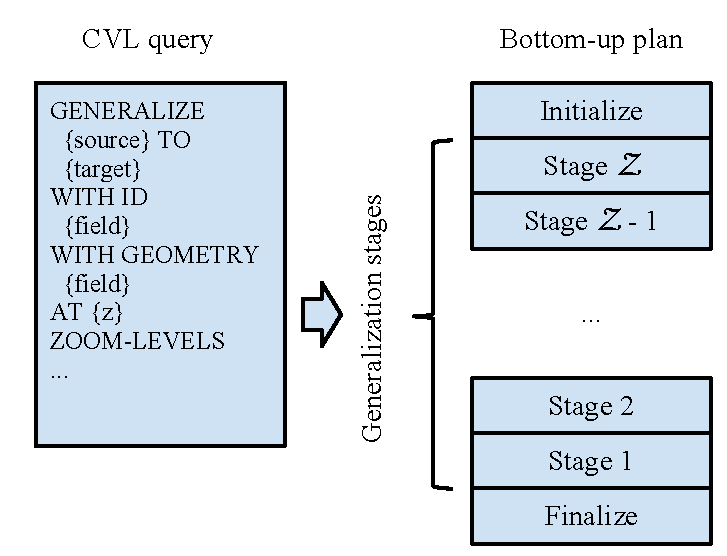
\includegraphics[scale=.7]{figs/cvl_compilation.pdf}
\caption{Compiling CVL to a bottom-up plan}
\label{fig:compilation}
\end{center}
\end{figure}

The bottom-up plan consists of three overall phases. A \emph{initialization} phase, a \emph{generalization} phase, and an \emph{finalization} stage. During the initializes phase the elements of the input are ranked and partitioned according to the CVL clauses for ranking and partitioning. During the generalization phase the constraints, transformations and forced levels are applied to the data. During the finalization stage the result set is assembled.

The generalization phase consists a $\mathcal{Z}$ stages, which are named after the zoom-levels. The stages are executed separately for each partition computed during the initialization phase. The bottom-up plan gets its name because it generalizes partitions starting with the highest scale (called Stage $\mathcal{Z}$), and ending with the lowest scale (called Stage $1$).

Let's consider the generalization phase for a single partition. The objective at each stage is to generalize the data in the partition for some zoom-level. Intuitively, the records that make it to the next stage, are the one that survived the generalization process at the previous stage. This implies that the records being processed a given stage are a subset of the records that were processed during the previous stage.

There are many algorithms that could be used to compute a stage. In this work we consider only one type of algorithm, namely an algorithm for the \emph{multi-hitting set problem}. The multi-hitting set problem and an several algorithms are covered in more detail in Section~\ref{sec:algorithms}. For now we simply state that there is a mapping from cartographic generalization to the hitting set problem.

\subsubsection{Sub-stages solve hitting set}
In this work we model the problem of generalizing records at a given zoom-level, by mapping to an instance of the multi-hitting set problem. This is implemented for each stage by performing five steps or sub-stages. This is shown in Figure~\ref{fig:stages}. 

As with the main stages, the output of a sub-stage is used as input to the next sub-stage.

\begin{figure}[htbp]
\begin{center}
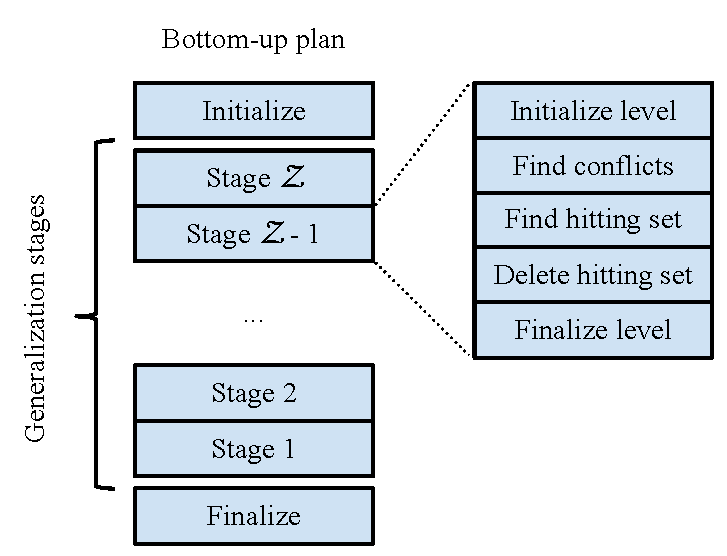
\includegraphics[scale=.7]{figs/cvl_stages.pdf}
\caption{Sub-stages of the bottom-up plan}
\label{fig:stages}
\end{center}
\end{figure}
